\documentclass[journal,a4paper,twocolumn]{IEEEtran}
\usepackage[T1]{fontenc}
\usepackage[utf8]{inputenc}
\usepackage{lmodern}
\usepackage{amsmath,amssymb,mathtools}
\usepackage{booktabs,array,graphicx}
\usepackage{placeins}
\usepackage[hidelinks]{hyperref}
\hypersetup{pdftitle={Optimal Driving Toward a Red Traffic Light},pdfauthor={Jan}}
\allowdisplaybreaks
\setlength{\emergencystretch}{2em}
\newcommand{\dd}{\,\mathrm{d}}
\newcommand{\CZK}{\mathrm{CZK}}
\newcommand{\cruise}{\mathrm{cr}}
\newcommand{\argmin}{\operatorname*{arg\,min}}
\newcommand{\ind}{\mathbf{1}}
\renewcommand{\topfraction}{0.95}
\renewcommand{\dbltopfraction}{0.95}
\renewcommand{\textfraction}{0.05}
\renewcommand{\floatpagefraction}{0.75}
\renewcommand{\dblfloatpagefraction}{0.75}
\setlength{\dbltextfloatsep}{8pt plus 1pt minus 2pt}
\setlength{\textfloatsep}{7pt plus 1pt minus 2pt}
\setlength{\abovecaptionskip}{4pt}
\setlength{\belowcaptionskip}{1pt}

\title{Optimal Driving Toward a Red Traffic Light\\[3pt]
\large Creating delay, preserving speed, and using switching-time information}
%\author{Jan}
\begin{document}
\maketitle

\begin{abstract}
A red light requires a driver to create delay, but the way that delay is created determines the position and speed available when green arrives. We study this tradeoff in a longitudinal vehicle model that minimizes travel-time and fuel cost, prohibits red crossing, and includes a downstream destination at a prescribed terminal speed. The deterministic cost of completing the journey gives an explicit economic value to speed at green. Under uncertain switching time, all realizations still observing red share one approach trajectory; a survival-weighted objective then determines when slowing is worthwhile. Numerical examples show early braking followed by coasting and pre-green speed recovery when the switch is known, and a shift toward later braking when early green is possible. Acceleration can also begin before the earliest possible green: in a narrow-prior example, allowing it lowers computed expected cost by about 0.0102 CZK. Realized information regret is largest near the broad-prior policy's transition into stopping. The computations identify locally optimized candidates in a stylized vehicle model.
\end{abstract}

\section{Introduction}
A driver travelling at 50 km/h sees a red light 300 m ahead. Cruising would reach the line in 21.6 s; in the model used here, free coasting would reach it in 25.30 s at 35.77 km/h. If green is known to arrive at 28 s, some braking is therefore unavoidable. Yet braking need not continue until green. Slowing early can create enough delay to permit acceleration near the end of the approach.

The reason is that the journey continues beyond the stop line. A useful approach must balance three quantities: time spent, fuel consumed, and the position and speed retained for the remaining journey. Braking early creates delay over a long interval. Accelerating later consumes some of that delay while restoring speed over a shorter interval. This makes a brake--coast--accelerate sequence a plausible candidate even while the signal remains red.

Uncertainty changes the timing of this exchange. If early green is possible, slowing immediately gives up an opportunity to proceed quickly. Preserving speed initially keeps that opportunity open, but may require stronger braking if red persists. Continued red is itself an observation: it eliminates earlier switching times and changes the remaining decision.

Probabilistic signal timing and optimal vehicle control have been studied in eco-driving and dynamic-programming formulations \cite{mahler,gaspard}. Here we use a tractable vehicle and fuel model to explain the allocation of delay. We first value the journey remaining after green, then formulate known and uncertain switching times, and finally compare the resulting trajectories. The numerical experiments address three questions: when should speed be sacrificed, can recovery start before green is possible, and at which realized switching times is advance information most valuable?

\section{Vehicle, route, and objective}\label{sec:model}
\subsection{Route and admissible motion}
The stop line is $x=0$, the start is $x=-D$, and the destination is $x=W$. Write $d=-x$ for distance to the line. The boundary conditions are
\begin{align}
 d(0)&=D=300\ \mathrm m, &v(0)&=v_{\max},\notag\\
 d(T_f)&=-W=-100\ \mathrm m, &v(T_f)&=v_{\max},
 \label{eq:init}
\end{align}
where $v_{\max}=50/3.6$ m/s and $T_f$ is the arrival time. Throughout the journey, $0\le v\le v_{\max}$.

The signal switches from red to green once, at time $S$, and remains green for the rest of the passage. Crossing on red is prohibited. Thus $d(t)\ge0$ before $S$; a vehicle reaching $d=0$ earlier must have $v=0$ and wait there. Reaching the line and waiting is distinct from crossing it. The finite-penalty extension is described in Appendix~\ref{app:fine}.

\subsection{Longitudinal dynamics}
Throttle $u$ and brake command $b$ lie in $[0,1]$. Their dynamics are
\begin{align}
 \dot d&=-v,\label{eq:dynamics_d}\\
 \dot v&=a_T(v)u-r(v)-a_b b,\label{eq:dynamics_v}\\
 a_T(v)&=\min\!\left\{\frac{A}{v+v_0},\ a_{\rm cap}+r(v)\right\},\label{eq:traction}\\
 r(v)&=r_0+k_Dv^2.\label{eq:road}
\end{align}
The road load includes rolling resistance and aerodynamic drag. The power-envelope parameters are
\begin{align}
 A=\frac{\eta_dP_e}{m}&=66.0\ \mathrm{m^2/s^3},\notag\\
 k_D=\frac{\rho C_DS_f}{2m}&=2.712966667\times10^{-4}\ \mathrm{m^{-1}},\notag\\
 r_0=C_{rr}g&=0.11772\ \mathrm{m/s^2}.
 \label{eq:mechpar}
\end{align}
The regularizer $v_0=1$ m/s removes the zero-speed singularity of the power approximation. The cap limits net full-throttle acceleration $a_T-r$ to $a_{\rm cap}=4.136672736$ m/s$^2$. Integrating the full-throttle model to 100 km/h gives 8.4 s. Within the entire 0--50 km/h range studied here the cap is active, so
\begin{equation}
 a_+(v):=a_T(v)-r(v)=a_{\rm cap}.
 \label{eq:aplus}
\end{equation}
Full braking adds $a_b=4$ m/s$^2$ to the road-load deceleration.

\begin{table}[!t]
\centering
\caption{Parameters of the illustrative vehicle model.}
\label{tab:car}
\begingroup\footnotesize\setlength{\tabcolsep}{3pt}
\begin{tabular}{@{}p{1.16in}p{0.80in}p{1.13in}@{}}
\toprule
Parameter & Value & Basis\\
\midrule
Engine rating $P_e$ & 110 kW & Octavia reference \cite{skoda}\\
Drag coefficient $C_D$ & 0.302 & Combi reference \cite{skoda}\\
Loaded mass $m$ & 1500 kg & Assumed\\
Wheel-power factor $\eta_d$ & 0.90 & Assumed\\
Frontal area $S_f$ & 2.20 m$^2$ & Assumed\\
Air density $\rho$ & 1.225 kg/m$^3$ & Assumed\\
Rolling coefficient $C_{rr}$ & 0.012 & Assumed\\
Regularizer $v_0$ & 1 m/s & Assumed\\
Net accel. cap & 4.137 m/s$^2$ & 8.4 s 0--100 fit\\
Brake addition $a_b$ & 4 m/s$^2$ & Assumed\\
\bottomrule
\end{tabular}\endgroup
\end{table}

Table~\ref{tab:car} defines an Octavia-inspired model. The source specification gives the 2.0 TDI 110 kW liftback an 8.4 s 0--100 km/h time and $C_D=0.294$, whereas the Combi has 8.5 s and $C_D=0.302$ \cite{skoda}. The present calculations combine the liftback acceleration benchmark with the Combi drag coefficient. They therefore describe an illustrative parameter set, not a reconstruction of one vehicle variant. The acceleration envelope is calibrated to one performance measurement; it does not resolve gears, engine speed, or traction limits separately.

For positive speed, $u=b=0$ means free coasting, and $u=0,b=1$ means full braking. Holding speed requires
\begin{equation}
 u_{\cruise}(v)=\frac{r(v)}{a_T(v)}.
 \label{eq:ucr}
\end{equation}
At rest the smooth numerical model uses force balance, $a_T(0)u-r_0-a_bb=0$, to hold $v=0$. One possible choice is $u=u_{\cruise}(0),b=0$; the transcription also admits simultaneous throttle and brake satisfying the same balance. These stationary commands are a mathematical convention. As shown below, all such balances incur only idle fuel at exact rest.

\subsection{Fuel use and running cost}
The cruise-fuel model comes from the companion reduced-speed-zone calculation \cite{companion}. The owner's moving-speed observations and idle rate are
\begin{equation}
\begin{array}{c|ccc}
3.6v\ (\mathrm{km/h})&9&80&130\\ \hline
\mathrm{FC}_{100}\ (\mathrm{L/100\,km})&10.0&5.0&6.5
\end{array},\qquad Q_0=0.6\ \mathrm{L/h}.
\label{eq:obs}
\end{equation}
The moving observations correspond to 0.9, 4.0, and 8.45 L/h. Interpolation through these points and the idle intercept gives
\begin{align}
 Q(v)&=Q_0+c_1v+c_2v^2+c_3v^3,\label{eq:Q}\\
 c_1&=0.120713517724,\notag\\
 c_2&=-0.000505754823921,\notag\\
 c_3&=0.0000881390936848,\notag
\end{align}
with $v$ in m/s and $Q$ in L/h.

To extend this steady-speed fit to varying throttle, put $q_{\cruise}=Q/3600$, $q_i=Q_0/3600$ in L/s, and use
\begin{equation}
 \dot f=q_i+\Gamma(v)u,\qquad
 \Gamma(v)=\frac{q_{\cruise}(v)-q_i}{u_{\cruise}(v)}.
 \label{eq:fuel}
\end{equation}
Here $f$ is cumulative fuel consumption. This construction reproduces $Q(v)$ at steady speed using the capped dynamics. During coasting and braking it assigns idle fuel use; at rest, $\Gamma(0)=0$. The affine dependence on throttle is a modeling assumption, rather than a measured transient fuel map, and omits overrun fuel cut.

Let $C_t$ denote the value of time in CZK/s and $c_f$ the fuel price in CZK/L. The running cost and objective are
\begin{align}
 \ell(v,u)&=C_t+c_f\bigl(q_i+\Gamma(v)u\bigr),\label{eq:ell}\\
 J&=\mathbb E\!\left[\int_0^{T_f}\ell(v,u)\dd t\right].
 \label{eq:objective}
\end{align}
The main examples use $C_t=300/3600$ CZK/s and $c_f=32$ CZK/L. Because the terminal speed is prescribed, an approach that leaves the car slow must also pay for subsequent recovery.

\section{The economic cost of creating delay}\label{sec:cost}
\subsection{Position and speed at green}
Once green is observed, only the remaining distance and current speed matter. For this model and the stated time valuations, the least-cost continuation is full throttle to $v_{\max}$ followed by cruise. Define the cost per metre of cruising at the cap,
\begin{equation}
 g_0=\frac{C_t+c_fq_{\cruise}(v_{\max})}{v_{\max}},
\end{equation}
and the recovery surcharge
\begin{equation}
 H(v)=\int_v^{v_{\max}}
 \frac{\ell(s,1)-g_0s}{a_+(s)}\dd s.
 \label{eq:H}
\end{equation}
The numerator subtracts the cruise cost of the distance covered while accelerating. The green continuation is consequently
\begin{equation}
 \boxed{\mathcal V_G(d,v)=g_0(d+W)+H(v).}
 \label{eq:VG}
\end{equation}
The first term values remaining distance; $H(v)$ is the additional cost of starting that continuation below the terminal speed. In particular, $H(v_{\max})=0$ and $H'(v)\le0$.

The required recovery distance is $(v_{\max}^2-v^2)/(2a_{\rm cap})$, at most 23.32 m. Since $W=100$ m, every admissible state before the line has enough remaining distance for this continuation. Increasing $W$ beyond that requirement adds cruise cost without changing the optimal red approach.

To verify optimality, write
\begin{equation}
 B(v)=C_t+c_fq_{\cruise}(v)-g_0v.
\end{equation}
For the fitted curve, cruise cost per metre decreases up to 50 km/h, so $B(v)\ge0$ on the permitted speed range. Substitution of \eqref{eq:H} gives
\begin{align}
 L_D(v,u,b)
 &:=\ell(v,u)-g_0v
 +H'(v)\bigl(a_T(v)u-r(v)-a_bb\bigr)\notag\\
 &=\frac{a_T(v)B(v)}{a_+(v)}(1-u)-a_bbH'(v)
 \ \ge0.
 \label{eq:delayrate}
\end{align}
Equality holds during full-throttle recovery and cruise at $v_{\max}$. Integrating $\ell+\dot{\mathcal V}_G=L_D\ge0$ to the destination, where $\mathcal V_G=0$, proves that no admissible continuation has lower cost than \eqref{eq:VG}.

\subsection{Known green time: where should delay be created?}\label{sec:known}
When $S=\tau$ is known, the red approach minimizes
\begin{equation}
 J_{\rm known}(\tau)=\int_0^\tau\ell(v,u)\dd t
 +\mathcal V_G(d(\tau),v(\tau))
 \label{eq:known}
\end{equation}
subject to the red-line constraint. It need not reach the line exactly at $\tau$; its task is to choose a useful position and speed at that time.

The same objective has a revealing alternative form:
\begin{equation}
 J_{\rm known}(\tau)
 =g_0(D+W)+\int_0^\tau L_D(v,u,b)\dd t.
 \label{eq:knowndelay}
\end{equation}
The constant term is the cost of an unobstructed journey at the speed cap. The nonnegative integral is the extra cost of the approach required by the red light. Thus the problem is to create the necessary delay at the least additional journey cost.

Coasting alone provides a useful benchmark. For $v_2<v_1$, its distance is
\begin{equation}
 D_c(v_1,v_2)=\frac{1}{2k_D}
 \ln\frac{r_0+k_Dv_1^2}{r_0+k_Dv_2^2}.
 \label{eq:coastdist}
\end{equation}
From the initial state it reaches the line in 25.30 s. Without braking, adding nonnegative throttle cannot delay this arrival. A known green at 28 s therefore requires some braking.

Braking early reduces distance covered throughout the following approach. This can create more delay than is ultimately needed, leaving room to rebuild speed before green. In \eqref{eq:delayrate}, full-throttle recovery has zero instantaneous excess cost relative to the green continuation, but consumes distance more quickly. Its timing is therefore governed by the delay already accumulated and the space remaining before the line. Section~\ref{sec:numerics} illustrates the resulting brake--coast--accelerate sequence.

\section{Uncertain switching time}\label{sec:feedback}
\subsection{One shared path while the signal remains red}
Let $S$ have density $f_S(t)$, distribution function $F_S(t)$, and survival probability $\bar F(t)=P(S>t)$. Observing red at time $t$ reveals $S>t$. With a fixed initial state, deterministic vehicle dynamics, and noiseless signal observations, all realizations still seeing red have the same observation history. They therefore follow one common path
\begin{equation}
 z_R(t)=(d_R(t),v_R(t)).
\end{equation}
When green occurs at $S=s$, the vehicle leaves that path and follows the optimal green continuation from $z_R(s)$. This constructs a causal policy for the specified initial state: decisions before the observed switch use no knowledge of its eventual time.

For $S\sim U(a,b)$, continued red truncates the original uniform distribution to the remaining interval. The switching hazard is
\begin{equation}
 \lambda(t)=\frac{f_S(t)}{\bar F(t)}
 =\begin{cases}
 0,&t<a,\\
 1/(b-t),&a\le t<b.
 \end{cases}
 \label{eq:hazard}
\end{equation}
The growing hazard expresses the increasing chance of green in the next short interval, conditional on red having persisted.

\subsection{Survival-weighted cost}
For a bounded switching-time support with upper endpoint $T_{\max}$, the expected cost of the common red path is
\begin{align}
 J_{\rm FB}
 &=\mathbb E\!\left[\int_0^S\ell(v_R,u_R)\dd t
 +\mathcal V_G(z_R(S))\right]\notag\\
 &=\int_0^{T_{\max}}\!\left[
 \bar F(t)\ell(v_R,u_R)+f_S(t)\mathcal V_G(z_R(t))
 \right]\dd t.
 \label{eq:survivalobjective}
\end{align}
Running cost is paid only on realizations still seeing red. The second term averages the continuation cost from the state at which green is observed.

Integration by parts yields the uncertain counterpart of \eqref{eq:knowndelay}:
\begin{equation}
 \boxed{J_{\rm FB}=g_0(D+W)+
 \int_0^{T_{\max}}\!\bar F(t)L_D(t)\dd t.}
 \label{eq:survivaldelay}
\end{equation}
Here $L_D(t)=L_D(v_R(t),u_R(t),b_R(t))$. The identity follows from $\dot{\bar F}=-f_S$, $\bar F(T_{\max})=0$, and $\dot{\mathcal V}_G=-g_0v+H'\dot v$. It connects the physical and statistical parts of the problem: deviations from the unobstructed journey are weighted by the probability that they will still be needed.

Delaying braking can avoid it altogether if green arrives first. If red persists, however, the available distance decreases and the eventual speed sacrifice may be greater. A prior excluding early green removes the first incentive and can favor creating delay earlier. These competing effects determine the common red path.

\begin{figure*}[!t]
\centering
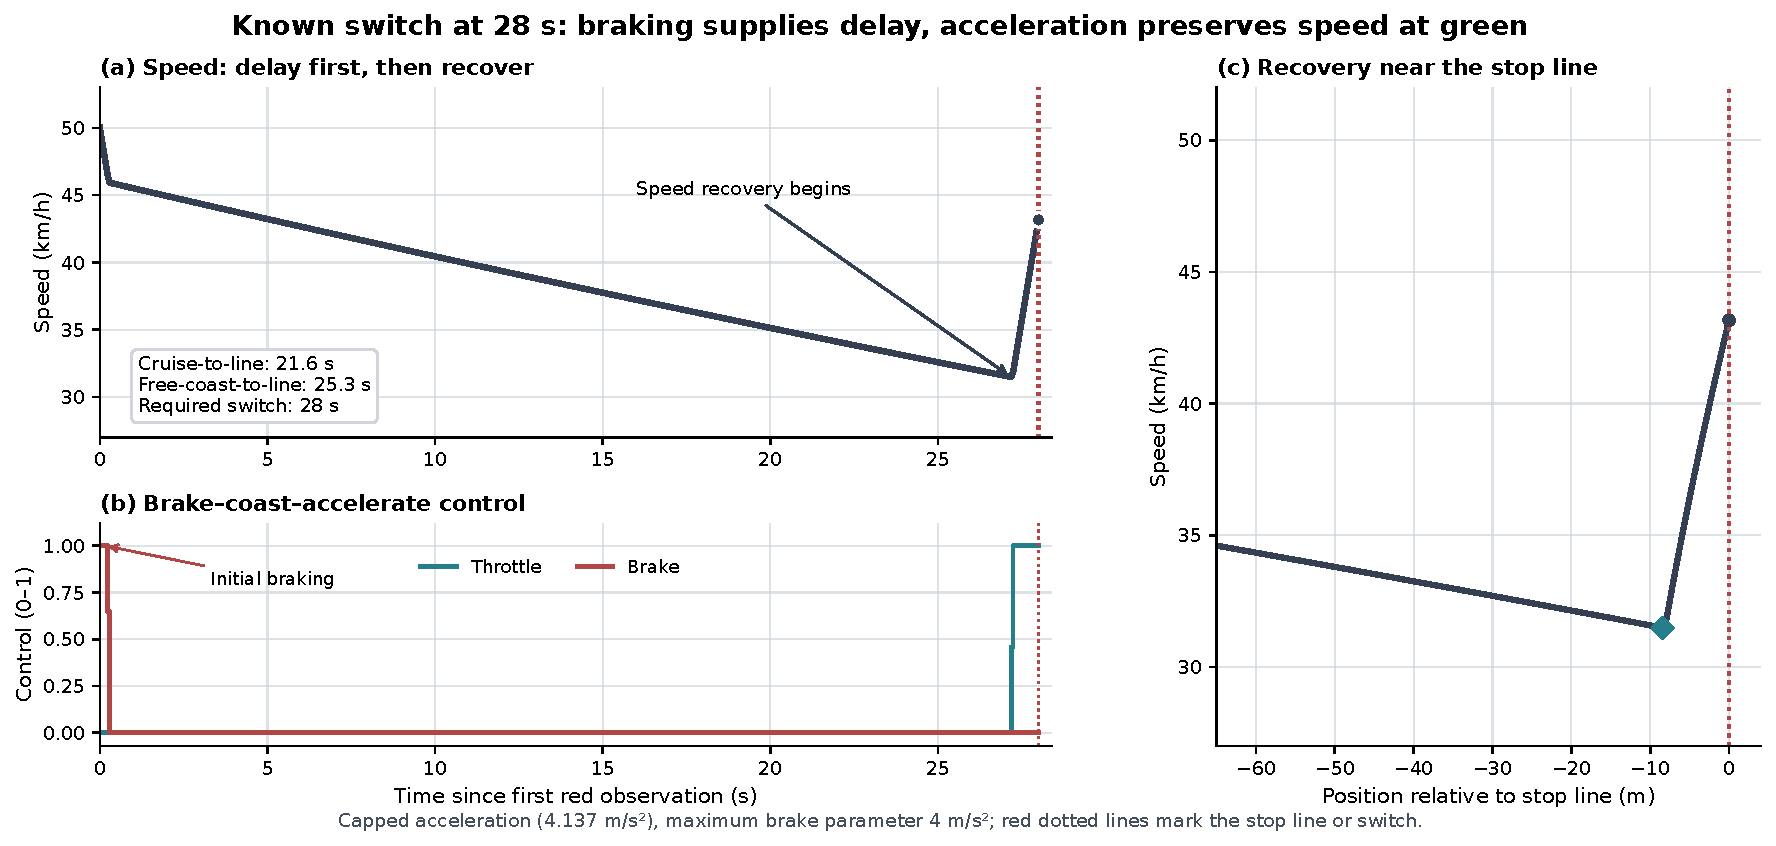
\includegraphics[width=.94\textwidth]{figures/fig1_known28_capped.pdf}
\caption{Known switching time $S=28$ s. Initial braking creates delay, coasting carries that delay through the approach, and acceleration beginning near 27.18 s restores speed before green. The vehicle reaches the line at the switch with about 43.16 km/h. Cruising and free coasting would arrive too early, at 21.6 and 25.30 s.}
\label{fig:known}
\end{figure*}

\subsection{Braking, coasting, and acceleration}
The conditional red value $\mathcal V_R(d,v,t)$ gives the corresponding local control structure. In the interior of the viable region it satisfies the piecewise-deterministic HJB equation \cite{davis,gaspard}
\begin{multline}
0=\partial_t\mathcal V_R+\min_{0\le u,b\le1}
\bigl\{\ell(v,u)-v\mathcal V_{R,d}\\
+(a_T(v)u-r(v)-a_bb)\mathcal V_{R,v}
+\lambda(t)(\mathcal V_G-\mathcal V_R)\bigr\}.
\label{eq:HJB}
\end{multline}
The numerical method optimizes the common red path directly using \eqref{eq:survivalobjective}; it does not compute a value map over all initial states.

Writing $p=\mathcal V_{R,v}$, the coefficients multiplying the controls are
\begin{equation}
 \Phi_u=c_f\Gamma(v)+a_T(v)p,\qquad
 \Phi_b=-a_bp.
 \label{eq:switch}
\end{equation}
At positive speed, away from singular arcs and state constraints, minimizing these affine terms gives
\begin{equation}
\begin{array}{c|c}
\text{Condition}&\text{Control}\\ \hline
p>0&u=0,\ b=1\quad\text{(brake)}\\
-c_f\Gamma/a_T<p<0&u=b=0\quad\text{(coast)}\\
p<-c_f\Gamma/a_T&u=1,\ b=0\quad\text{(accelerate)}.
\end{array}
\label{eq:modes}
\end{equation}
Positive $p$ means extra speed would increase remaining cost; sufficiently negative $p$ makes traction worth its fuel cost. Coasting occupies the interval between these thresholds.

A switch occurs when a coefficient crosses zero. The value function can remain smooth throughout this change \cite{liberzon}. Intermediate controls can occur on a state constraint or singular arc; an intermediate command in a single transcription cell can also represent a cell containing a switch. It is not, by itself, evidence for a sustained partial-braking phase.

At the speed cap, controls must prevent further acceleration. At $d=0$ before green, the vehicle must be stationary and remain there. At a finite upper support endpoint, the red value approaches $\mathcal V_G$ from admissible states as the remaining red interval vanishes.

\section{Numerical results}\label{sec:numerics}
All experiments use the model in Table~\ref{tab:car}, $D=300$ m, $W=100$ m, and $c_f=32$ CZK/L. The default time valuation is 300 CZK/h. The reported trajectories are the least-cost feasible candidates found by multistart direct transcription; numerical checks and their scope are collected in Section~\ref{sec:sensitivity}.

\subsection{Known switch: create delay early, recover speed late}
Figure~\ref{fig:known} fixes $S=28$ s. The trajectory brakes at the start, coasts for most of the approach, and accelerates from approximately 27.18 s. Its minimum speed is about 31.48 km/h; it reaches the line at green with 43.16 km/h. The total journey cost is 3.6755 CZK.

Early braking supplies the delay that coasting alone cannot provide. Because the lower speed persists over most of the approach, only a short braking interval is needed. Near green, the vehicle uses the remaining distance to recover speed. The example shows that a green later than the free-coasting arrival need not force a stop: the necessary delay can instead be accumulated while rolling.



\subsection{Uncertain switch: when should speed be sacrificed?}
Figure~\ref{fig:info} compares policies for $U(0,60)$ and $U(26,30)$ s, emphasizing the same realized switch $S=28$ s. Brown curves show the path followed only while red continues; green branches begin when green is actually observed. The dashed reference knows $S=28$ in advance.

The broad prior leaves open the possibility of early green. Its policy preserves more speed initially: at 10 s it carries 44.09 km/h, compared with 38.49 km/h under the late prior; at 20 s the corresponding speeds are 38.57 and 33.28 km/h. If red persists, the broad-prior policy begins braking near 24 s and stops at the line. For the realization $S=28$ it must then restart. The late-prior policy creates delay earlier and is still rolling when green arrives, at 29.30 km/h and about 16 m before the line.

\begin{figure*}[!t]
\centering
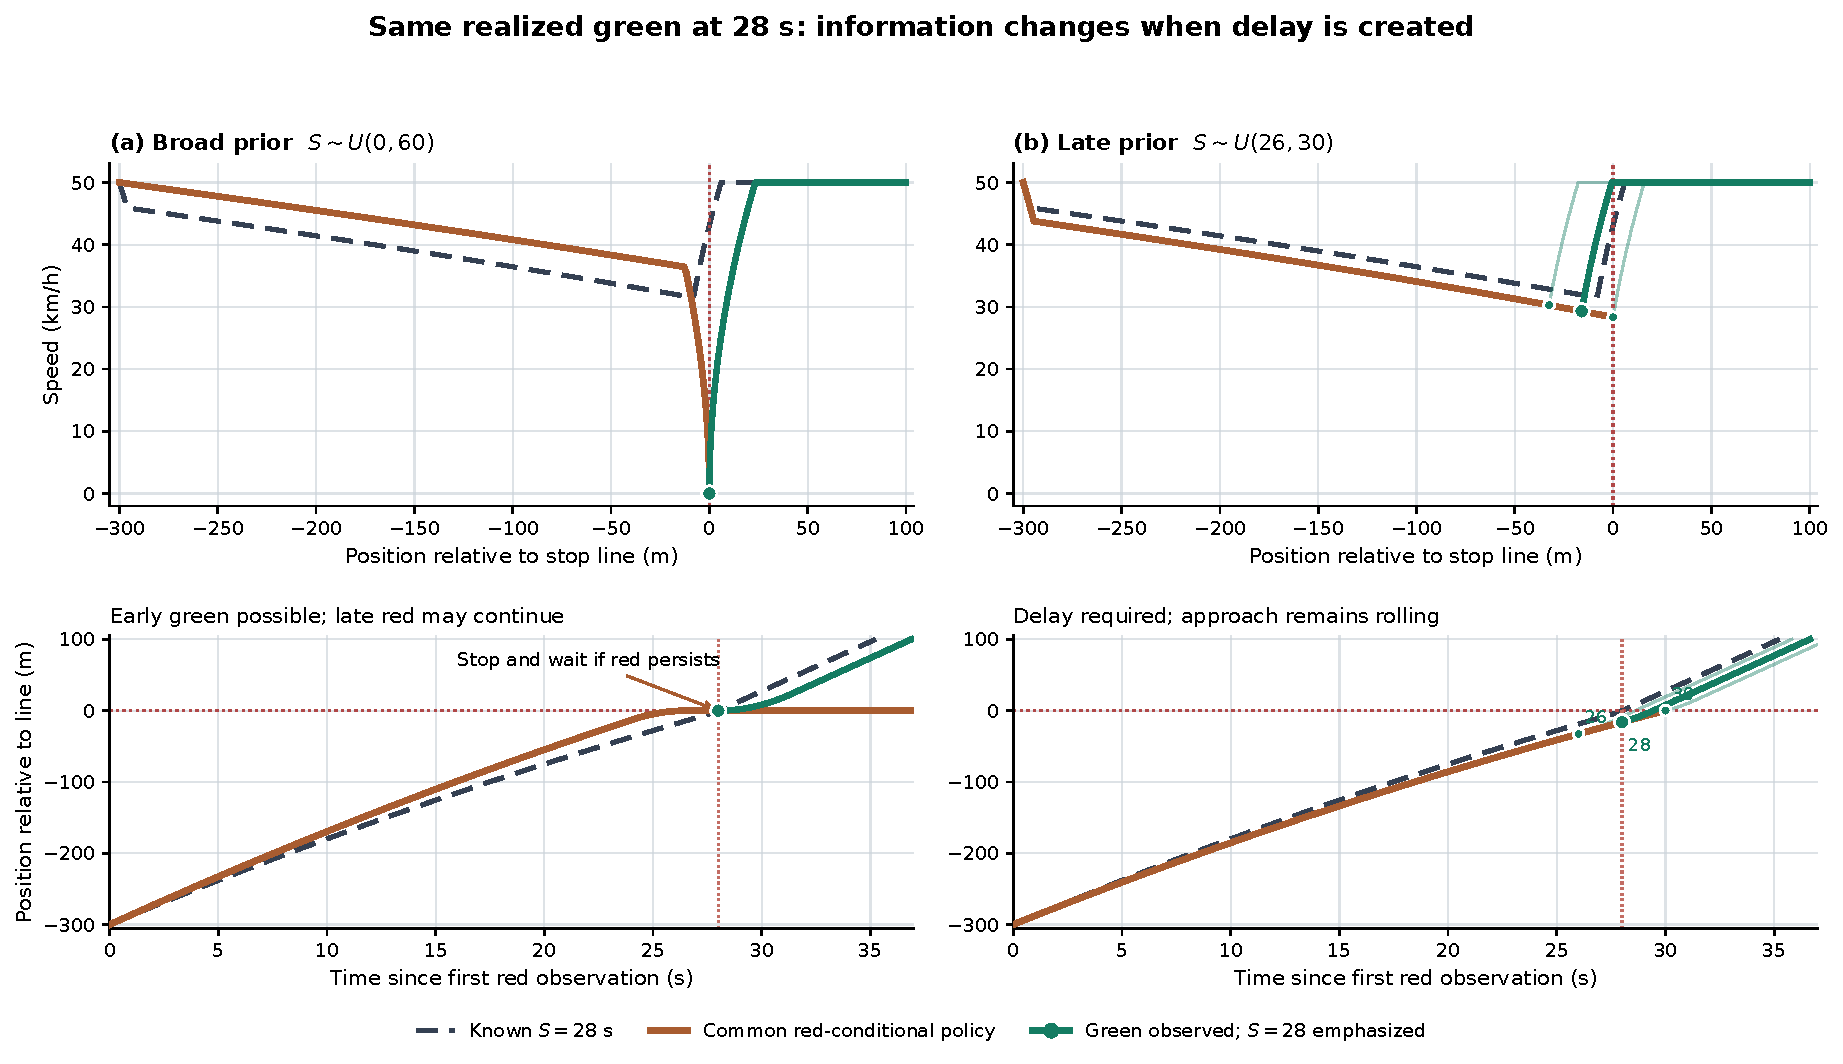
\includegraphics[width=.94\textwidth]{figures/fig2_information_capped.pdf}
\caption{Allocation of delay under different information. Dashed charcoal: known $S=28$ s. Brown: common path conditional on continued red. Green: continuation after observing green, with $S=28$ emphasized and $S=26,30$ also shown for the late prior. The broad prior preserves speed initially but stops under prolonged red; the late prior produces a rolling approach. After a branch point, the continuing brown curve represents other realizations still observing red.}
\label{fig:info}
\end{figure*}

For this shared realization, total costs are 3.6755 CZK with exact knowledge, 3.8499 CZK with late-prior feedback, and 4.1331 CZK with broad-prior feedback. Table~\ref{tab:realized} separates the physical consequences. The broad-prior restart costs both time and fuel; late-prior feedback stays closer to the deterministic reference, but still arrives later and uses more fuel.

\begin{table}[!t]
\centering
\caption{Same realized green at 28 s: state at green and completed journey. Arrival times are measured from the start; fuel totals are model estimates derived from the saved trajectories.}
\label{tab:realized}
\begingroup\footnotesize\setlength{\tabcolsep}{4pt}
\begin{tabular}{@{}lrrrr@{}}
\toprule
Information & $d(S)$ & $v(S)$ & $T_f$ & Fuel\\
 & (m) & (km/h) & (s) & (mL)\\
\midrule
Known $S=28$ & 0.00 & 43.16 & 35.23 & 23.11\\
$U(26,30)$ & 16.01 & 29.30 & 36.64 & 24.89\\
$U(0,60)$ & $\approx0$ & $\approx0$ & 36.88 & 33.12\\
\bottomrule
\end{tabular}\endgroup
\end{table}

These priors describe different opportunities, not a controlled change in uncertainty width: their means and both support endpoints differ. The supported conclusion is that allowing early green shifts speed sacrifice later. Expectations under the two different priors do not by themselves measure the value of better information.

\subsection{Anticipation: accelerate before green is possible}\label{sec:anticipation}
For a more stringent test of anticipation, take $S\sim U(27,27.5)$ s and raise the time valuation to 900 CZK/h. The narrow support concentrates green near a known time, while the higher time valuation makes speed recovery more valuable. Figure~\ref{fig:anticipatory} shows acceleration beginning in the cell starting at 26.425 s, before any green is possible.

The mechanism is the same as in the deterministic example. Delay has already been created; the vehicle can recover speed while remaining behind the line throughout the guaranteed-red interval. This action uses the prior distribution, not advance knowledge of the realized switch.

To measure the contribution of this behavior, reoptimize with
\begin{equation}
 u(t)\le u_{\cruise}(v(t)),\qquad t<27\ \mathrm s,
 \label{eq:noinc}
\end{equation}
on the still-red branch. This permits maintaining or reducing speed before 27 s and leaves acceleration unrestricted thereafter. Thus the comparison isolates the permission to begin speed recovery before the earliest possible green.

\begin{figure*}[!t]
\centering
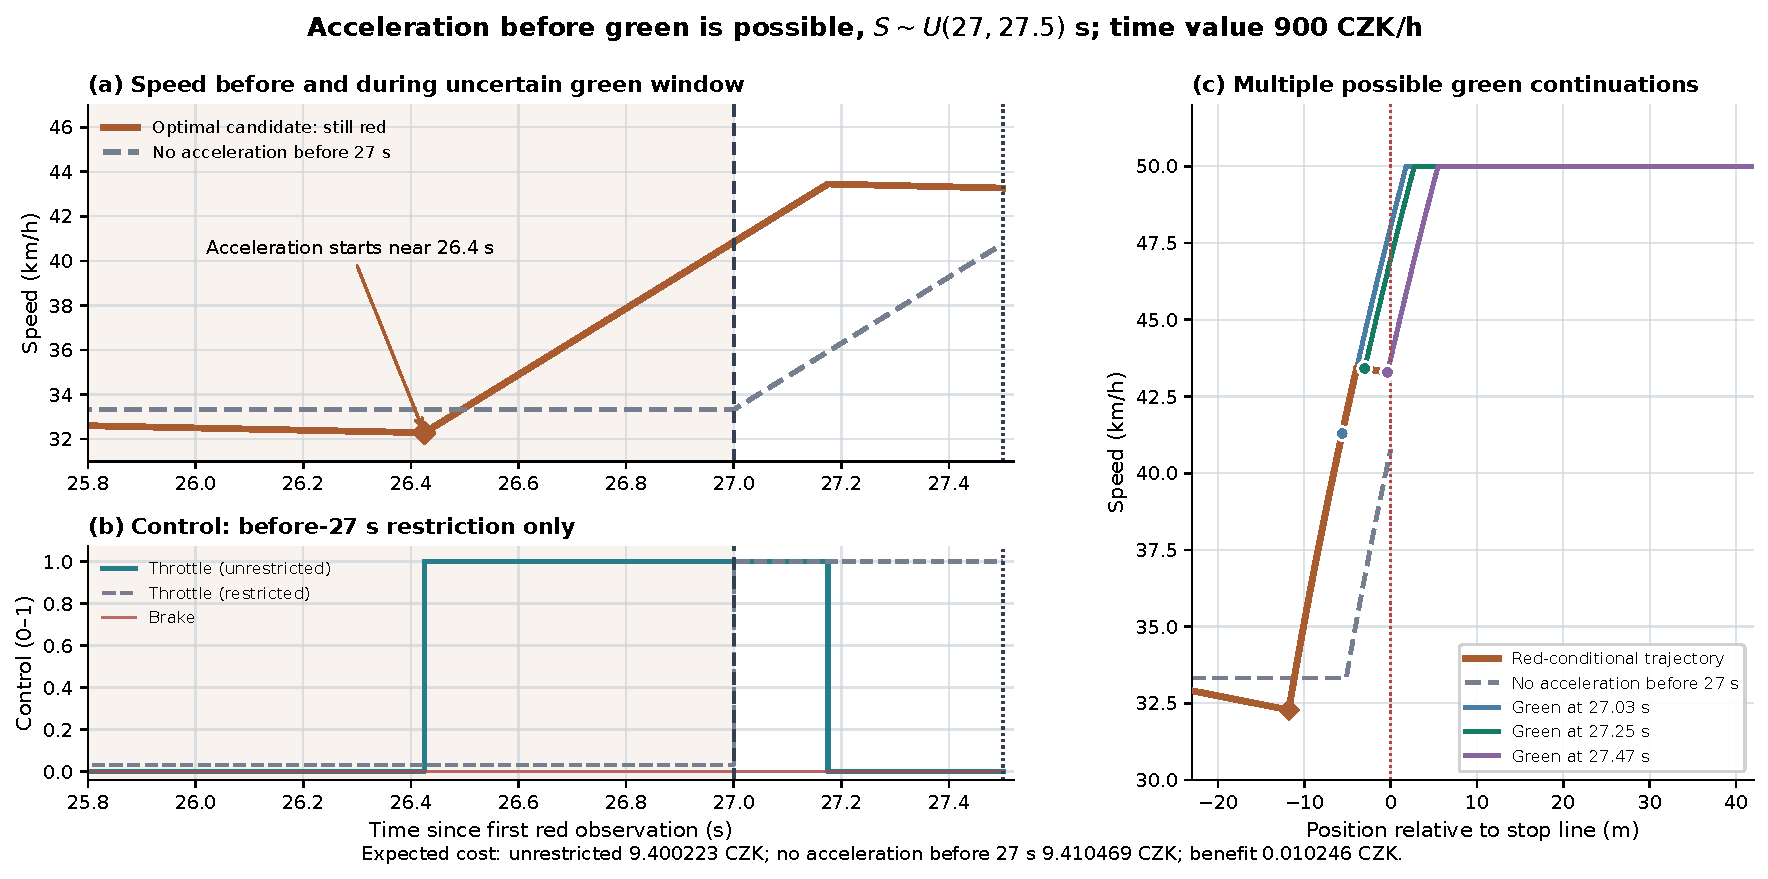
\includegraphics[width=.94\textwidth]{figures/fig3_anticipation_capped.pdf}
\caption{The figure demonstrates that for certain  parameters, acceleration can occur before green light triggers. It happens if the driver knows he is nearing the last possible switching moment. $S\sim U(27,27.5)$ s and $C_t=900$ CZK/h (chosen high for the pattern to appear). Brown: unrestricted common red path. Gray dashed: reoptimized path with speed-increasing throttle prohibited only before 27 s. Other colors show continuations after green observations at 27.03, 27.25, and 27.47 s. The pre-27 s acceleration permission lowers computed expected cost by about 0.0102 CZK.}
\label{fig:anticipatory}
\end{figure*}

\begin{table}[!t]
\centering
\caption{Cost of prohibiting pre-27 s acceleration for $U(27,27.5)$; 1,100 cells, costs in CZK.}
\label{tab:anticipation}
\begingroup\footnotesize\setlength{\tabcolsep}{3pt}
\begin{tabular}{@{}rccc@{}}
\toprule
$C_t$ (CZK/h) & Unrestricted & Restricted & Difference\\
\midrule
300 & 3.615398 & 3.616782 & 0.001385\\
900 & 9.400223 & 9.410469 & 0.010246\\
\bottomrule
\end{tabular}\endgroup
\end{table}

Table~\ref{tab:anticipation} gives the computed differences. At 900 CZK/h, permitting anticipation reduces cost by about 0.11\%; at 300 CZK/h the benefit is approximately 0.00138 CZK. These small effects establish a numerical mechanism within the model. Their practical magnitude depends on assumptions about transient fuel use, acceleration, and comfort.

\subsection{Information value: the cost of being wrong about timing}
A value-of-information comparison holds the prior fixed. For a feedback policy optimized under that prior, let $J_{\rm FB}(s)$ be its realized journey cost when green occurs at $s$, and let $J_{\rm known}^{\star}(s)$ be the optimal cost with $s$ known in advance. Then
\begin{align}
 R(s)&=J_{\rm FB}(s)-J_{\rm known}^{\star}(s),\notag\\
 \mathrm{VOI}&=\mathbb E[R(S)]
 =\int R(s)f_S(s)\dd s.
 \label{eq:regret}
\end{align}
Exact optimization would give $R(s)\ge0$, since a driver knowing $s$ could always reproduce the feedback trajectory. Numerically, the deterministic reference is the least-cost feasible local candidate found at each sampled switching time. The plotted regret and VOI are estimates based on those references.

Figure~\ref{fig:regret} shows that the value of information is concentrated around particular decisions. Under the broad prior, regret first rises because the feedback vehicle coasts while a driver knowing an early green could maintain speed. It then falls as the known green becomes late enough to require slowing too. Around the feedback policy's braking and stopping transition, regret rises sharply and peaks near 26.5 s at about 0.505 CZK. A switch then arrives after speed has been sacrificed, making the restart costly.

For still later switches, broad-prior regret declines: it is about 0.236 CZK at 40 s and 0.135 CZK at 60 s. Longer red also requires the informed driver to create substantial delay, narrowing the advantage of exact timing. The deterministic reference remains rolling in these cases, with minimum speeds of about 17.75 and 4.90 km/h, respectively. Thus the largest regret occurs near the transition into stopping, rather than at the longest red duration.

\begin{figure*}[!t]
\centering
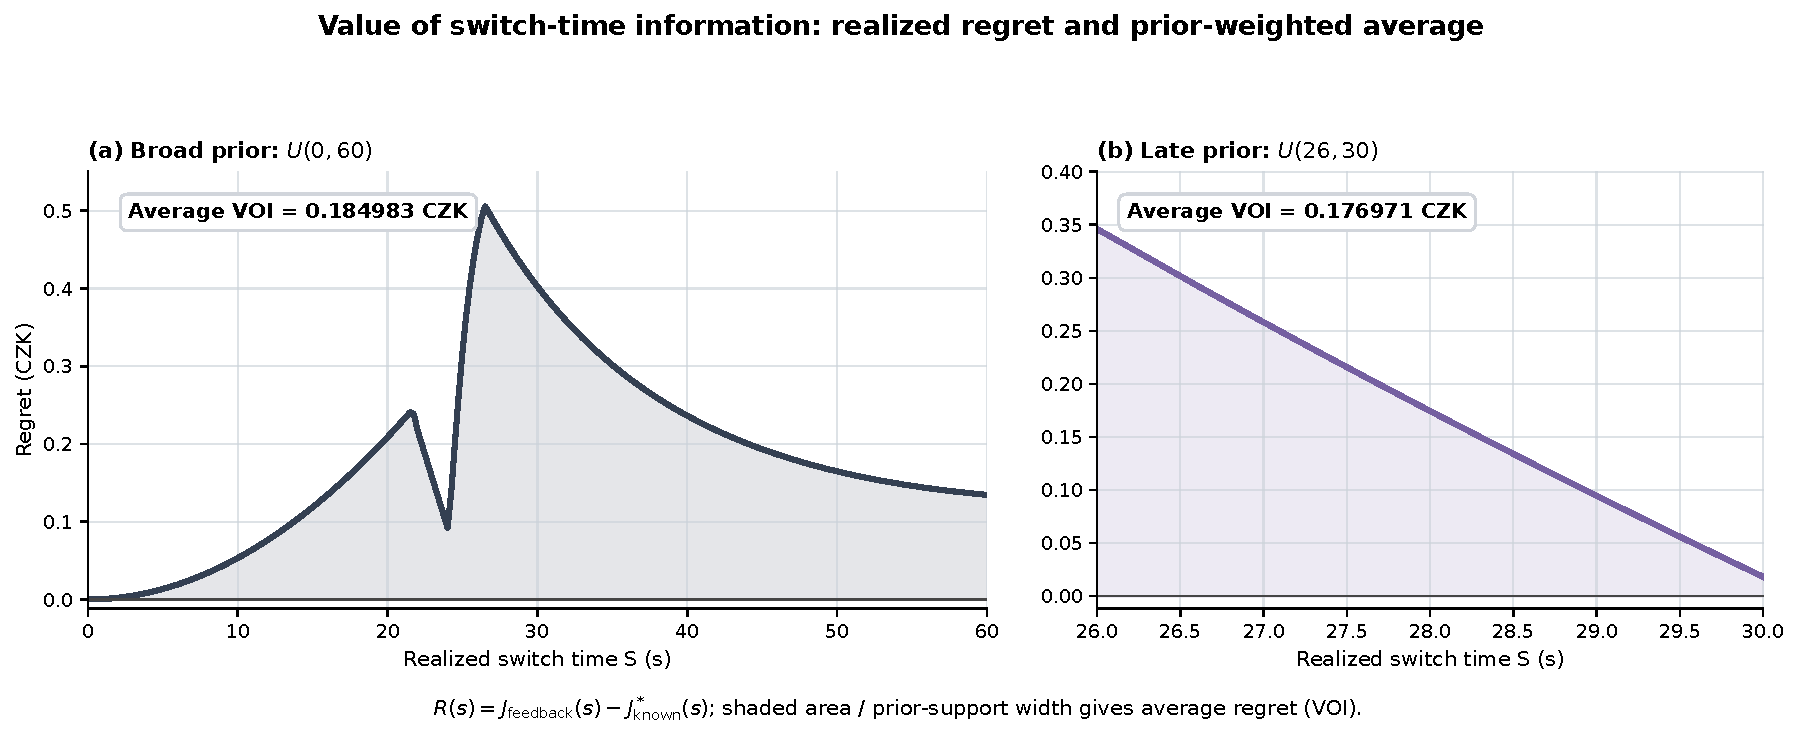
\includegraphics[width=.94\textwidth]{figures/fig4_regret_capped.pdf}
\caption{Realized regret relative to the known-switch reference. Under the broad prior, the largest loss occurs near the braking-to-stop transition, followed by decreasing regret for later green. Under the late prior, regret decreases across the support. For each uniform prior, shaded area divided by support width gives its estimated VOI. References use multistart deterministic solutions and shape-preserving cubic interpolation between sampled switching times.}
\label{fig:regret}
\end{figure*}

For the late prior, regret decreases across the support. Its policy is prepared for red to persist until 30 s; an earlier switch exposes the cost of delay that hindsight would have made unnecessary. Table~\ref{tab:voi} averages regret within each prior. Estimated VOI is 0.185 CZK for $U(0,60)$ and 0.177 CZK for $U(26,30)$. Their similar averages conceal quite different patterns of realized regret.

\begin{table}[!t]
\centering
\caption{Expected cost with and without perfect switching-time information, and their difference (CZK).}
\label{tab:voi}
\begingroup\footnotesize\setlength{\tabcolsep}{4pt}
\begin{tabular}{@{}lccc@{}}
\toprule
Prior & Perfect info. & Feedback & VOI\\
\midrule
$U(0,60)$ & 4.278768 & 4.463751 & 0.184983\\
$U(26,30)$ & 3.673528 & 3.850498 & 0.176971\\
\bottomrule
\end{tabular}\endgroup
\end{table}

\section{Numerical evidence and model scope}\label{sec:sensitivity}
The transcription uses piecewise-constant controls, fourth-order Runge--Kutta dynamics, and nodal and intermediate-stage feasibility checks. Cell survival integrals and switching masses are exact; state-dependent costs use approximate midpoints. IPOPT uses rolling and stopping initializations, with neighboring-solution continuation for deterministic reference sweeps.

The deterministic information reference uses 480 cells, sampled switching times, and shape-preserving cubic interpolation. The broad and late feedback policies use 480 and 360 cells, respectively. The narrow-prior comparison uses 1,100 cells with a node exactly at 27 s. Its pre-27 s benefit changes from 0.010238 CZK at 550 cells to 0.010246 CZK at 1,100 cells for 900 CZK/h; the corresponding values at 300 CZK/h are 0.001388 and 0.001385 CZK. A deterministic 60 s check changes from 6.835906 CZK at 480 cells to 6.835871 CZK at 960 cells.

The archived realization-based integration agrees with the feedback objectives within $2.8\times10^{-6}$ CZK for the broad prior and $2.6\times10^{-8}$ CZK for the late prior. That calculation reuses the transcription states and running-cost approximation, so it checks consistency of the expectation calculation. Separate continuous-dynamics reintegration of the known-28 s path, both feedback paths, and the four 1,100-cell anticipation paths reproduces their costs within $5\times10^{-6}$ CZK. This supports evaluation of the saved policies; it does not bound the improvement available from a different policy.

Multistart and mesh checks do not certify global optimality or total VOI error. A difference of locally optimized values is neither an upper nor a lower bound on true VOI. Extra digits in the tables identify the calculations, rather than the accuracy of the vehicle model.

The main physical limitation is transient fuel extrapolation: cruise observations and one acceleration time do not validate fuel use during braking and recovery. Other omissions include comfort and jerk, reaction time, queues and following vehicles, gradients, observation noise, and overrun fuel cut.

The archive includes an alternative uncapped model with a larger brake parameter, 7 m/s$^2$. It reproduces the qualitative examples but gives different VOIs. Since both acceleration and braking differ, this comparison establishes sensitivity to combined mechanical assumptions; attributing it to the acceleration cap alone would require a comparison at fixed braking strength. A study of uncertainty width would likewise require a controlled family of priors.

\section{Conclusion}
Approaching a red light requires allocating delay while preserving position and speed for the remaining journey. The green continuation values the state at the switch; uncertainty weights the additional cost of the red approach by the probability that it is still needed.

Early braking can create room for coasting and speed recovery before a known green. When early green is possible, preserving speed initially can be preferable, at the risk of an eventual stop. With sufficiently concentrated timing information, recovery can begin even before green is possible. In the broad-prior example, exact information is most valuable near the transition into stopping, rather than for the longest red duration. These mechanisms are the central results of the model.

\appendices
\section{Finite penalties for crossing on red}\label{app:fine}
A finite expected sanction can be added as a crossing event. If $T_\times$ denotes the time the vehicle crosses the line and $K=p_{\rm enforce}F_{\rm fine}$, the extended objective is
\begin{equation}
 J=\mathbb E\!\left[\int_0^{T_f}\ell(v,u)\dd t
 +K\ind\{T_\times<S\}\right].
 \label{eq:finiteobjective}
\end{equation}
Reaching the line and waiting at rest incurs no sanction. A red crossing attaches the outgoing value $K+\mathcal V_G(0,v)$ to that boundary; it does not add a penalty rate to the interior HJB. All numerical experiments prohibit this option.

\begin{thebibliography}{9}
\bibitem{companion}
Jan, \emph{A Cost Model for Driving Through a Reduced-Speed Zone: Measured Fuel Use and a Tractable Transition Model for a \v{S}koda Octavia}, companion manuscript.

\bibitem{skoda}
\v{S}KODA AUTO, \emph{\v{S}KODA OCTAVIA Press Kit}, 2017, 2.0 TDI 110 kW performance and body specifications for the liftback and Combi.
\href{https://cdn.skoda-storyboard.com/2017/02/170207-\%C5\%A0KODA-OCTAVIA-Tiskov\%C3\%A1-mapa.pdf}{Press kit (PDF)}.

\bibitem{mahler}
G. Mahler and A. Vahidi, ``An optimal velocity-planning scheme for vehicle energy efficiency through probabilistic prediction of traffic-signal timing,'' \emph{IEEE Trans. Intelligent Transportation Systems}, vol.~15, no.~6, pp.~2516--2523, 2014, doi:10.1109/TITS.2014.2319306.

\bibitem{gaspard}
M. E. Gaspard and A. Vladimirsky, ``Optimal Driving Under Traffic Signal Uncertainty,'' \emph{IFAC-PapersOnLine}, vol.~55, no.~16, pp.~25--31, 2022, doi:10.1016/j.ifacol.2022.08.076.

\bibitem{liberzon}
D. Liberzon, \emph{Calculus of Variations and Optimal Control Theory: A Concise Introduction}. Princeton University Press, 2012, Ch.~5 and Secs.~4.4.2--4.4.3.
\href{https://liberzon.csl.illinois.edu/teaching/cvoc.pdf}{Online text (PDF)}.

\bibitem{davis}
M. H. A. Davis, \emph{Markov Models and Optimization}. London, U.K.: Chapman \& Hall, 1993.
\end{thebibliography}
\end{document}
